The first data on the cost to fix defects as a function of lifecycle phase date back to large systems in the late 70s from IBM~\cite{Fagan76}, TRW~\cite{Boehm76}, GTE~\cite{Daly77}, and Bell Labs~\cite{Stephenson76} (Figure~\ref{fig:cost-to-fix}). These studies suggest that the cost (in terms of effort) to find and fix an error monotonically increases with lifecycle phase. For large projects, the ratio of cost-to-fix in the requirements phase to cost-to-fix in operation is on the order of 1:100. Furthermore, cost function is superlinear, with the greatest rates of increase in the acceptance testing and operations phases.

\begin{figure}
 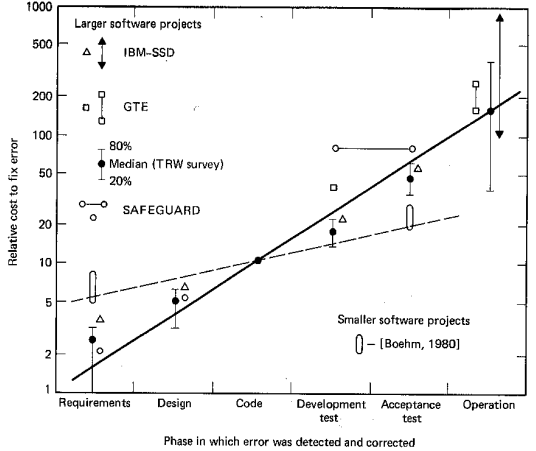
\includegraphics[width=3.3in]{boehm_cost-to-fix.png}
 \caption{Cost-to-fix curve. From~\cite{Boehm81}.}\label{fig:cost-to-fix}
 \end{figure}
 
In the 40 years since these initial studies, few studies have been published on the cost-to-fix curve as a function of lifecycle phase. Boehm~\cite{Boehm80} provides data suggesting that the cost-to-fix curve for small projects (from two student projects of 2000 deliverable source instructions) is flatter than for large projects (the dashed line of Figure~\ref{fig:cost-to-fix}). Shull et al.~\cite{Shull02} conducted a literature survey and held a series of e-workshops with industry experts on fighting defects. Workshop participants from Toshiba and IBM reported cost-to-fix ratios of 1:137 and 1:117 for large projects respectively~\cite{Shull02} -- the raw data points are not provided. One notable example to the traditional cost-to-fix curve is the CCPDS-R described by Royce~\cite{Royce98}: a million-line, safety-critical missile defense system (Figure~\ref{fig:royce}). In this project, design changes (including architecture changes) required approximately twice the effort of implementation and test changes, and the cost-to-fix in implementation and test phases increased slowly. Boehm~\cite{Boehm10} attributes this success to the CCPDS-R development process, which focused on removing architecture risk early in the devleopment lifecycle.

\begin{figure}
 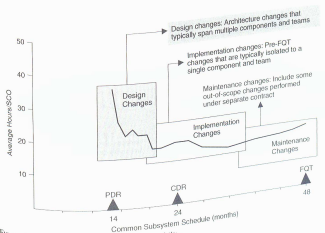
\includegraphics[width=3.3in]{Royce98.PNG}
 \caption{Exception to the rule - CCPDS-R cost-to-fix curve. From~\cite{Royce98}.}\label{fig:royce}
 \end{figure}
 
As discussed earlier, one goal of agile methods is to flatten the cost-to-change curve~\cite{beck00}. Relatively little empirical data exists on this point. Clutterbuck et al.~\cite{Clutterbuck09} studied 5-month effort by a small-to-medium enterprise team developing a 71KLOEC web interface to a database application to implement 18 change requests (Figure~\ref{fig:clutterbuck}). Note that these were for new and changed user requirements, not defects. Clutterbuck et al. found the cost of change to be relatively flat until the later phases, with much of the effort spent in analysis of the change requests~\cite{Clutterbuck09}. Elssamadisy and Schalliol~\cite{Elssamadisy02} anecdotally report on the growing, high cost of rework in a 50 person, three-year, 500KLOEC Extreme Programming project as the project grew in size and complexity.

\begin{figure}
 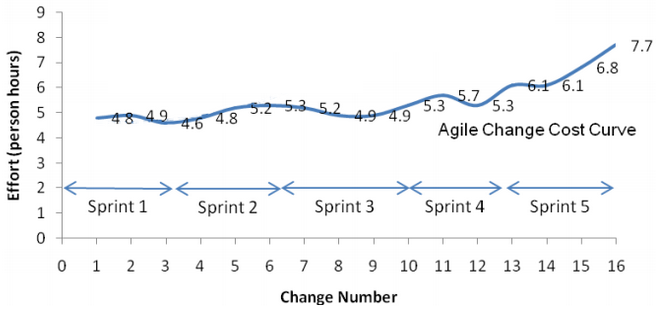
\includegraphics[width=3.3in]{clutterbuck.png}
 \caption{Cost of change from an agile case study~\cite{Clutterbuck09}.}\label{fig:clutterbuck}
 \end{figure}
 
 We note that previous work focuses on cost-to-fix as a function of lifecycle phase irrespective of when the defect was injected, that is, previous work analyzes the cost to fix a defect found in test regardless of whether that defect was a requirements error or a coding mistake. To our knowledge, our research represents the first large-scale study of phase delay as a contributor to the cost-to-fix curve.